\documentclass[10pt]{article}
\usepackage[utf8]{inputenc}
\usepackage{epsfig}
\usepackage{verbatim}
\usepackage{ulem}
\usepackage{lscape}
\usepackage{multicol}
\usepackage{graphics}
%\usepackage{graphicx}
\usepackage{amssymb}
\usepackage{fancyhdr}
\usepackage{fancybox}
\usepackage[table]{xcolor}
\usepackage[T1]{fontenc}
%\usepackage{caption}
\usepackage{subcaption}
\usepackage{hyperref}
\usepackage{url}
%\usepackage{setspace}
%\usepackage{float}
\usepackage{listings}

\bibliographystyle{plain}

\usepackage[a4paper]{geometry}
\geometry{top=1.8in, bottom=1.8in, left=1.5in, right=1.5in}

\setlength{\parindent}{0in}
\setlength{\parskip}{3mm}

% http://www.elec.ucl.ac.be/logistique/informatique/Digests/TeX/1999/texhax.04
\setcounter{secnumdepth}{5}   % depth of section numbering
\setcounter{tocdepth}{5}      % depth of section showing in TOC

\newcommand{\includeSVG}[1]{
  \includegraphics[scale=1.0]{figs/#1.pdf}
}
\newcommand{\textdesc}[1]{\textit{\textbf{#1}}} % font for \descitem
\newcommand{\descitem}[1]{\item \textdesc{#1}}

% Default fixed font does not support bold face
\DeclareFixedFont{\ttb}{T1}{txtt}{bx}{n}{10} % for bold
\DeclareFixedFont{\ttm}{T1}{txtt}{m}{n}{10}  % for normal

% Custom colors
\usepackage{color}
\definecolor{deepblue}{rgb}{0,0,0.5}
\definecolor{deepred}{rgb}{0.6,0,0}
\definecolor{deepgreen}{rgb}{0,0.5,0}

% Python style for highlighting
\newcommand\pythonstyle{\lstset{
  language=Python,
  basicstyle=\ttm,
  otherkeywords={self, map},             % Add keywords here
  keywordstyle=\ttb\color{deepblue},
  emph={MyClass,__init__},          % Custom highlighting
  emphstyle=\ttb\color{deepred},    % Custom highlighting style
  stringstyle=\color{deepgreen},
  frame=tb,                         % Any extra options here
  showstringspaces=false            % 
}}

% Python environment
\lstnewenvironment{python}[1][]
{
\pythonstyle
\lstset{#1}
}
{}

\title{SimBuilding, the Manual\\\scalebox{0.85}{a Discrete Event Simulator for Building Modeling}}
\author{Aslak Johansen \url{aslj@itu.dk}\\Matias Bjørling \url{mabj@itu.dk}\\Javier González González \url{jgon@itu.dk}}

\begin{document}

\maketitle
%\abstract{This paper briefly describes the SimBuilding simulator. Both the internal models and the interface is covered.}
\tableofcontents
\newpage

%%%%%%%%%%%%%%%%%%%%%%%%%%%%%%%%%%%%%%%%%%%%%%%%%%%%%%%%%%%%%%%%%%%%%%%%%%%%%%%%%%%%%%%%%%%%%%%%%%%%%%%%%%%%%%%%%%%%%%%%
%%%%%%%%%%%%%%%%%%%%%%%%%%%%%%%%%%%%%%%%%%%%%%%%%%%%%%%%%%%%%%%%%%%%%%%%%%%%%%%%%%%%%%%%%%%%%%%%%%%%%%%%%%%%%%%%%%%%%%%%
%%%%%%%%%%%%%%%%%%%%%%%%%%%%%%%%%%%%%%%%%%%%%%%%%%%%%%%%%%%%%%%%%%%%%%%%%%%%%%%%%%%%%%%%%%%%%%%%%%%%%%%%%%%%%%%%%%%%%%%%


%%%%%%%%%%%%%%%%%%%%%%%%%%%%%%%%%%%%%%%%%%%%%%%%%%%%%%%%%%%%%%%%%%%%%%%%%%%%%%%%%%%%%%%%%%%%%%%%%%%%%%%%%%%%%%%%%%%%%%%%
%%%%%%%%%%%%%%%%%%%%%%%%%%%%%%%%%%%%%%%%%%%%%%%%%%%%%%%%%%%%%%%%%%%%%%%%%%%%%%%%%%%%%%%%%%%%%%%%%%%%%%%%%%%%%%%%%%%%%%%%
%%%%%%%%%%%%%%%%%%%%%%%%%%%%%%%%%%%%%%%%%%%%%%%%%%%%%%%%%%%%%%%%%%%%%%%%%%%%%%%%%%%%%%%%%%%%%%%%%%%%%%%%%%%%%%%%%%%%%%%%


\section{Introduction}

% context, the modern building: sensors, actuators
Modern buildings incorporate a wide array of sensors and actuators. They are typically connected by a primitive ruleset. Examples could include:
\begin{itemize}
  \item \textbf{if} rain \textbf{then} window.close()
  \item \textbf{if} room[3].temp < 20 \textbf{then} room[3].heater.state(ON)
  \item \textbf{if} room[0].motion(last 30 min) \textbf{then} room[3].light.state(OFF)
\end{itemize}

% motivation: why write code for a building?
In a time when people are starting to realize the impact of climate change legislation has been introduced in order to limit the use of fossil fuels. A significant amount of the energy used today is spent in buildings. Still, little is known about how buildings are used and the tolerances of the factors influencing the experience of the occupants. With experience in these areas we can make informed decisions about the tradeoffs involved in running a building.

% testing: testbed,simulation
Buildings a complex systems with multiple layers of controllable services. Writing code for such a system requires a considerable amount of testing. It is paramount that the software controlling the building not turn off the electricity during normal operation. The same goes for water, ventilation, heating and cooling. For this reason many rely on full-scale building testbeds. This is obviously an expensive solution. The alternative is to \textsl{simulate} the building, and with it comes compromises.

\begin{figure}[hb]
  \begin{subfigure}[b]{0.5\textwidth}
    \centering
    \rotatebox{0}{\scalebox{0.6}{\includeSVG{buildinglogic}}}
    \caption{Real building}
    \label{fig:interfacing:real}
  \end{subfigure}
  \begin{subfigure}[b]{0.5\textwidth}
    \centering
    \rotatebox{0}{\scalebox{0.6}{\includeSVG{simulatorlogic}}}
    \caption{Simulated building}
    \label{fig:interfacing:sim}
  \end{subfigure}
  
  \caption{Interfacing real and simulated buildings.}
  \label{fig:interfacing}
\end{figure}

% the simulator: discrete event simulator
This paper describes the setup of a discrete event building simulator and the limitations it brings. The simulator steps through time in discrete steps. For each step it calculates the state of the building based on the prior state, the temporal increment and any pending actions. The idea -- as illustrated in figure \ref{fig:interfacing} -- is to provide an interface similar to that of a real building so that code can be moved to a real-world deployment with a minimal amount of modification.

% layout of paper
In section \ref{sec:internals} we describe the internal workings of the simulator at a high level. In section \ref{sec:interface} we describe two levels of interfaces to the simulator. For the high-level interface we list requirements and give instructions for installation. In section \ref{sec:lessons} we write about the lessons we learned during the development of this simulator.

%%%%%%%%%%%%%%%%%%%%%%%%%%%%%%%%%%%%%%%%%%%%%%%%%%%%%%%%%%%%%%%%%%%%%%%%%%%%%%%%%%%%%%%%%%%%%%%%%%%%%%%%%%%%%%%%%%%%%%%%
%%%%%%%%%%%%%%%%%%%%%%%%%%%%%%%%%%%%%%%%%%%%%%%%%%%%%%%%%%%%%%%%%%%%%%%%%%%%%%%%%%%%%%%%%%%%%%%%%%%%%%%%%%%%%%%%%%%%%%%%
%%%%%%%%%%%%%%%%%%%%%%%%%%%%%%%%%%%%%%%%%%%%%%%%%%%%%%%%%%%%%%%%%%%%%%%%%%%%%%%%%%%%%%%%%%%%%%%%%%%%%%%%%%%%%%%%%%%%%%%%

\section{Internal Configuration}
\label{sec:internals}

% intro
The simulator models a building and provides the means to interact with it. Buildings are modeled as systems made up of subsystems. Some of these subsystems rely on models of external phenomena. Figure \ref{fig:layers} illustrates a simple building model with subsystems illustrated as \textsl{layers}.

\begin{figure}[htb]
  \begin{center}
    \rotatebox{0}{\scalebox{0.4}{\includeSVG{layers}}}
  \end{center}
  \caption{Examples of relationships between layers, objects and models.}
  \label{fig:layers}
\end{figure}

% layer
Each layer models some property of relevance to the concept of a building. This modeling is typically done through graphs of objects. A layer is a model for which we provide increased visibility. Instead of only exposing the result, a layer exposes the logic behind the result.

% granularity

% timeline
The timeline of the building is driven by simulator inputs and models of relevant phenomena. Examples of these include occupancy and cloud cover.

\subsection{The Temporal Dimension}

In the simulator time is measured in seconds and a year is 365 days. There is no concept of dates, leap-years or leap-seconds. The simulation is performed at discrete intervals (aka the \textsl{stepsize}) and all datapoint values represent this particular interval. As a result incrementing the interval will cause accumulated values to increase.

\subsection{Objects}

% this section allows us to serialize the description
Most simulated objects interact with multiple layers. This section provides a short functional description of the relevant objects. Objects have static properties and dynamic properties. In this section we will stick to the static properties as these are the ones which needs to be set up during the initial phase. The simulator will spin without access to the dynamic properties. The dynamic properties are discoverable.

\subsubsection{Generators}

The generators consume petrol which is stored in tanks. They have to be primed in order to be capable of turning on. Turning a generator on \textsl{unprimes} it. The priming process needs to be done manually in real-life but we allow it to be done through software for the simulation. The following properties define that translation process:
\begin{itemize}
\descitem{Capacity} How much energy the generator produces when on.
\descitem{Efficiency} A scale for how much electrical energy is generated per unit of gas.
\end{itemize}

\subsubsection{Solar panels}

Solar panels converts sunlight into electrical energy. The following property define that translation process:
\begin{itemize}
\descitem{Efficiency} A scale for how much electrical energy is generated per photonic energy. This maps to the product of panel efficiency and panel size.
\end{itemize}

\subsubsection{Batteries, tanks and basins}

Storage container for electrical energy, water or gas. Each have the following associated properties:
\begin{itemize}
\descitem{Capacity} How much it can hold.
\end{itemize}

\subsubsection{Heaters and Air-conditioners}

Both heaters and air-conditioners are modeled using the following properties
\begin{itemize}
  \descitem{Wattage} The energy consumed when fully on.
  \descitem{Efficiency} A scale for how much heat is generated/removed per watt.
  \descitem{Gain} A float value in the range [0;1] for how much it is on. At 1 it consumes the maximum wattage.
\end{itemize}

\subsubsection{Lamps}

Lamps consume electrical energy in order to produce light. The following properties define that translation process:
\begin{itemize}
\descitem{Wattage} How much energy the lamp consumes when fully on.
\descitem{Gain} A float value in the range [0;1] for how much it is on. At 1 it consumes the maximum wattage.
\descitem{Efficiency} A scale for how much light is generated per watt.
\end{itemize}

\subsubsection{Blinds}

Blinds consume electrical energy in order to change state. The following properties define the operation process:
\begin{itemize}
\descitem{Speed} How fast the binds change state.
\descitem{Efficiency} A scale for how much energy is required to change the state.
\end{itemize}

\subsection{Models}

\subsubsection{Sun Model}
\label{sec:internals:models:sun}

The sun is modeled as a double sine. The one sine has a yearly period with minimum on the change of the year. The other sine has a daily period with minimum at midnight.

\subsubsection{Cloud Model}
\label{sec:internals:models:cloud}

Clouds a modeled as random patterns with added noise. This is subtracted from the sun in order to get temperature and light. This affects temperature and solar panel production.

\subsubsection{Rain Model}
\label{sec:internals:models:rain}

The rain model is derived from the cloud cover. Nothing fancy here. It affects the rain collection.

\subsubsection{Occupancy Model}
\label{sec:internals:models:occupancy}

The occupancy model is sadly, very limited. It simply provides an occupancy indication at the granularity of the building. The occupancy is linked to the water consumption.

\subsubsection{Grid Model}
\label{sec:internals:models:grid}

A grid model is used to simulate the service dropout on the electric grid. It has two parameters; maximum uptime $t_{\mathrm{up, max}}$ and maximum downtime $t_{\mathrm{down, max}}$. A change of state will trigger the scheduling of the next change of state. The delay is a random number between 0 and the relevant maximum time.

\subsubsection{Mains Model}
\label{sec:internals:models:mains}

A model of the water mains is used to simulate service failure in the water mains. It is implemented in the exact same way as the grid model.

\subsection{Layers}

\subsubsection{Occupancy Layer}

The occupancy layer delegates its responsibility to the occupancy model described in section \ref{sec:internals:models:occupancy}.

\subsubsection{Environmental Layer}

The environment layer consists of models for sun (section \ref{sec:internals:models:sun}), rain (section \ref{sec:internals:models:rain}) and cloud cover (section \ref{sec:internals:models:cloud}).

\subsubsection{Hydro Layer}

% basics
The hydro layer models flows of water. Figure \ref{fig:hydro} shows the default configuration of the hydro layer. Water is distributed through a hub modeled as a multiplexer. Inputs can come from either the water mains or a basin which is stores collected rain water. Whenever it rains water flows into the basin.

\begin{figure}[htb]
  \begin{center}
    \rotatebox{0}{\scalebox{0.4}{\includeSVG{defaulthydro}}}
  \end{center}
  \caption{Default setup of hydro layer.}
  \label{fig:hydro}
\end{figure}

% consumption
In the standard setup water is consumed according to a consumption model which is essentially
\begin{eqnarray}
  \nonumber V = c_1 \cdot \mathbf{occupancy} + c_2
\end{eqnarray}

% blackout
A simple blackout model has been implemented for the water mains. If the water multiplexer does not receive enough water on the active input its output will be turned off. This will cause the taps to stop functioning and the water requirements of the building to cease to be met.

\subsubsection{Energy Layer}

% basics
At the energy layer we model the flow and conversion of energy. Figure \ref{fig:energy} shows the default configuration of the energy layer. Electrical energy is distributed through a hub modeled as a multiplexer. Inputs can come from three sources; two generators of different capacity and a solar panel. Each input is buffered using a battery.  The output of the solar panel is dependent of the solar cycle and the cloud cover.

\begin{figure}[htb]
  \begin{center}
    \rotatebox{0}{\scalebox{0.4}{\includeSVG{defaultenergy}}}
  \end{center}
  \caption{Default setup of energy layer.}
  \label{fig:energy}
\end{figure}

% blackouts
A simple grid blackout model has been implemented. The functionality of lamps, blinds heaters and air-conditioners is depending on the availability of electrical power.

\subsubsection{Thermal Layer}

At the thermal layer the building is modeled as a room adjacency graph. Nodes represents rooms, heaters, aircons and the outside environment. The heat distribution is essentially modeled through successive overrelaxation of the edges at a granularity of 0.1 second, independently of the temporal granularity of the rest of the simulation. Each edge is associated with a thermal conductivity factor in the range of [0;1]. These values are chosen to prevent positive feedback in the simulation.

\subsubsection{Light Layer}

% basics
Light is simulated at a per-room basis. It is calculated as
\begin{eqnarray}
  \nonumber L = \sum_{i=0}^{all} \mathbf{lamps}[i] + \sum_{i=0}^{all} \left(\mathbf{has\_blinds}[i] ~?~ \mathbf{blinds}[i] : 1\right) \cdot \mathbf{windows}[i] \cdot \mathbf{cloud} \cdot \mathbf{sun}
\end{eqnarray}
where $\mathbf{blinds}[i]$ is a factor in the range of [0;1] defining how much light is allowed to pass through the window of size $\mathbf{windows}[i]$. The metric is more-or-less the combined photonic energy in the room. Distribution and spectrum of light is not simulated.

%%%%%%%%%%%%%%%%%%%%%%%%%%%%%%%%%%%%%%%%%%%%%%%%%%%%%%%%%%%%%%%%%%%%%%%%%%%%%%%%%%%%%%%%%%%%%%%%%%%%%%%%%%%%%%%%%%%%%%%%
%%%%%%%%%%%%%%%%%%%%%%%%%%%%%%%%%%%%%%%%%%%%%%%%%%%%%%%%%%%%%%%%%%%%%%%%%%%%%%%%%%%%%%%%%%%%%%%%%%%%%%%%%%%%%%%%%%%%%%%%
%%%%%%%%%%%%%%%%%%%%%%%%%%%%%%%%%%%%%%%%%%%%%%%%%%%%%%%%%%%%%%%%%%%%%%%%%%%%%%%%%%%%%%%%%%%%%%%%%%%%%%%%%%%%%%%%%%%%%%%%

\section{Interface}
\label{sec:interface}

The core simulator model is accessible through a low-level interface. This requires manual stepping. We add a high-level interface that keeps the core \textsl{alive} so that it can be interfaced as if it was a real building. Time is accelerated though.

\subsection{Low-level Interface}

We won't go into details regarding the low-level interface. There is a demo of a 3 room building available at \texttt{/bisp/sim/buildings/demo.py} within the repository. Figure \ref{fig:demo} shows a plot of a 7 day simulation on this building.

\begin{figure}[htb]
  \begin{center}
    \rotatebox{0}{\scalebox{1.0}{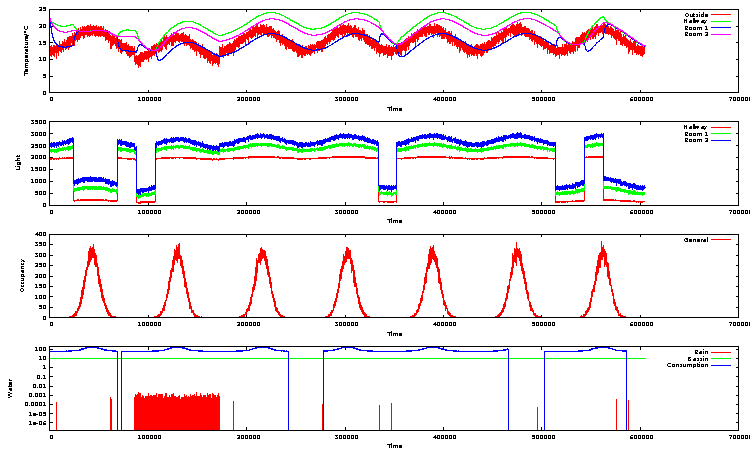
\includegraphics[scale=1.0]{figs/demo_temp.pdf}}}
  \end{center}
  \caption{Sample run of the demo without any actuation.}
  \label{fig:demo}
\end{figure}

\subsection{High-level Interface}

%TODO: Matias: Please describe the restfull interface here.

To be filled out

Needs to reference figure \ref{fig:interface:mediumlevel}

\begin{figure}[htb]
  \begin{center}
    \rotatebox{0}{\scalebox{1.0}{\includeSVG{mediumleveloverview}}}
  \end{center}
  \caption{Medium-level overview of the system around the high-level interface.}
  \label{fig:interface:mediumlevel}
\end{figure}

\subsubsection{Requirements}

%TODO: Matias: Which packages and DBMS are needed?

To be filled out
\begin{itemize}
  \descitem{django} (the D is silent)
  \descitem{tastypie}
  \descitem{networkx}
  \descitem{apscheduler}
  \descitem{mysql} For storing time-series data of the simulations.
\end{itemize}

\subsubsection{Installation}

%TODO: Matias: How should it be set up?

To be filled out

\subsubsection{Example Building}

We provide an example building. Figure \ref{fig:building:example} illustrates the layout. There are three types of rooms:
\begin{enumerate}
  \descitem{Hallways} Have no windows but 5 lamps, 2 heaters and 2 air-conditioners. Rooms 6, 13 and 20 are hallways.
  \descitem{Bathrooms} Have no windows but 2 lamps and 1 water tap\footnote{The water tap is not implemented. Instead there is a building-granularity consumption model.}. Rooms 5, 12 and 19 are bathrooms.
  \descitem{Ordinary} Have 2 lamps, 2 windows with blinds, 1 heater and 1 air-conditioner. All other rooms are ordinary rooms.
\end{enumerate}

\begin{figure}[htbp]
  \begin{center}
    \rotatebox{0}{\scalebox{1.0}{\includeSVG{building0}}}
  \end{center}
  \caption{Blueprint of the example building.}
  \label{fig:building:example}
\end{figure}

\subsubsection{Adding Buildings}

%TODO: Javier: How does one add buildings?

To be filled out

%%%%%%%%%%%%%%%%%%%%%%%%%%%%%%%%%%%%%%%%%%%%%%%%%%%%%%%%%%%%%%%%%%%%%%%%%%%%%%%%%%%%%%%%%%%%%%%%%%%%%%%%%%%%%%%%%%%%%%%%
%%%%%%%%%%%%%%%%%%%%%%%%%%%%%%%%%%%%%%%%%%%%%%%%%%%%%%%%%%%%%%%%%%%%%%%%%%%%%%%%%%%%%%%%%%%%%%%%%%%%%%%%%%%%%%%%%%%%%%%%
%%%%%%%%%%%%%%%%%%%%%%%%%%%%%%%%%%%%%%%%%%%%%%%%%%%%%%%%%%%%%%%%%%%%%%%%%%%%%%%%%%%%%%%%%%%%%%%%%%%%%%%%%%%%%%%%%%%%%%%%

\section{Lessons Learned}
\label{sec:lessons}

\subsection{Granularity}

The big question when writing a building simulator is what should be simulated and -- just as important -- at which granularity. We did not have this discussion. As a result the occupancy model became underdeveloped and the lack of predictability resulted in structural overhead.

\subsection{Metrics}

One of the lessons learned was that the simulator should use -- and respect -- real metrics. This means that the unit of water consumption is L, the flow of energy is J/s and so on. It also means that the calculations should be correct.

\subsection{Building Representation}

A physical representation of the building is needed for humans to relate to it. Revit provides this.

A logical representation of the building is needed for simulation. This can include
\begin{itemize}
  \descitem{Room adjacency graph} Which rooms share walls. This is needed for simulation the thermal behavior of the building.
  \descitem{Room connectivity graph} Which rooms share doors. This is needed for occupant behavior modeling. See section \ref{lessons:occupancy}.
  \descitem{Energy distribution graph} How is the energy distribution graph constructed. Note that it should be modeled as a graph -- not a tree -- for the general case.
  \descitem{Water distribution graph} How is the energy distribution graph constructed. This is very similar to the energy distribution graph.
  \descitem{Models} for sun, rain, clouds, occupancy and so on.
\end{itemize}

Some objects needs to be part of both representations, others should be it.

\subsection{Occupancy Modeling}
\label{lessons:occupancy}

The current occupancy model is very primitive and lacks resolution. What we want is per-room granularity and predictability. For this to work we need a room connectivity graph to model how an occupant can move from one room to another, and a per-occupant agent to model the movement of individual occupants. The logic of these agents could potentially be generated from real-world traces. This level of realism would allow building logic to perform preemptive actions across space. The current model only allows us to do that across time.

\subsection{Repeatability}

% motivation
A key use case for simulators is to enable users to compare multiple implementations. In a simulator we have the opportunity to make sure that two runs generate the exact same conditions for the client software. This is among other things used for verifying that adding a feature has no negative side-effects.

% how
There are two things that can break this. The first is if the simulator relies on some live data, like weather stations. We are not doing this. The second is models relying on random generators. We have a few of these. By allowing the users to seed the generator with a known value we can ensure a fixed sequence of random numbers and that will provide repeatability.

\subsection{Testability}

% HAL testing
A building exists in an environment which follows a yearly cycle. Testing control-logic should be 

\subsection{Trace-based Modeling}

% motivation: model realism

% how: gathering, interpolation (sinc), Nyquist

% example: climograph interpolation

\subsection{Cross-layer Communication}

Layers needs to be connected. A lamp appears in both the light layer and the energy layer. An electric heater appears in both the thermo layer and the energy layer. Values from the models also needs to be pushed into the relevant layers. Figure \ref{fig:lessons:xlayer} illustrates a rather clean way of implementing these connections.

\begin{figure}[htb]
  \begin{center}
\begin{python}
# setup layers
layer1 = Layer1()
layer2 = Layer2()

# setup connections
connections = []
connections.append(lambda : Layer1.set_value(Layer2.get_value()))

# actuate connections
map(lambda e: e(), connections)
\end{python}
  \end{center}
  \caption{Python code for pulling and pushing data between objects.}
  \label{fig:lessons:xlayer}
\end{figure}

\subsection{Development Efficiency}

Project planning is key to keeping the development efficiency high when 3+ people from different schools of thought are working on the same project.

\end{document}

